\section{Generalization \& Regularization}
\subsection{Overfitting}
\begin{itemize}
    \item A model that perfectly fits the data does not have to be perfect
    \item In-Sample Error (Trainig error) was minimized (MSE = 0)
    \item Out-of-sample Error (Generalization Error, Test Error) is the MSE of new Data
    \item A good model has a low Generalization Error
    \item Overfitting happens if the MSE of Training Error is small thanks to a complex model but the Generalization Error is large
\end{itemize}
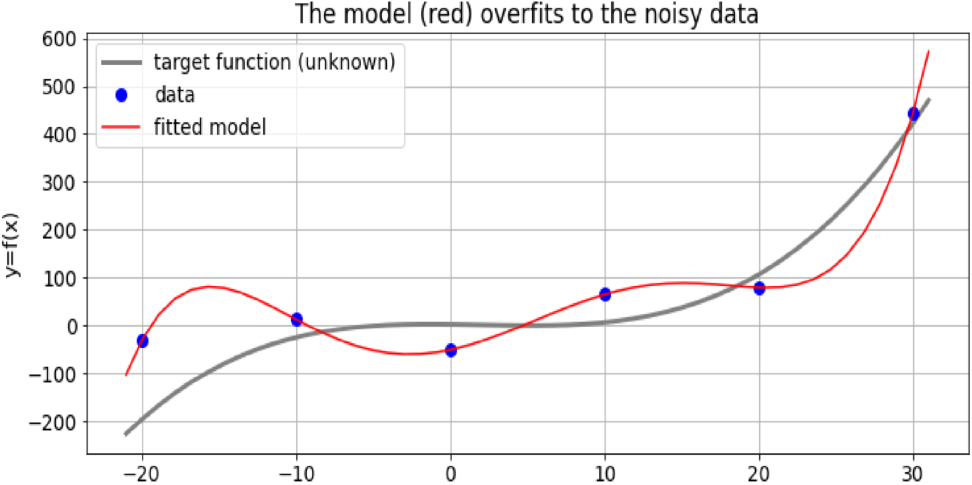
\includegraphics[width=0.9\linewidth]{overfitting.png}

\subsection{Underfitting}
\begin{itemize}
    \item Using a too simple model
    \item In-Sample Error is large
    \item Generalization Error is large
\end{itemize}

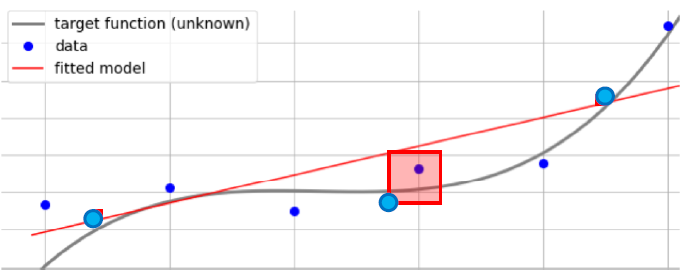
\includegraphics[width=0.9\linewidth]{underfitting.png}

\subsection{Training-Set, Test-Set, Model Evaluation}
\begin{itemize}
    \item The Generalization Error can't be calculated
    \item But Estimated
    \item Split the data into 2 sets
    \begin{itemize}
        \item Training-Set (~80\% of data)
        \item Test-Set (~20\% of data)
    \end{itemize}
\end{itemize}
\textbf{Training:}
\begin{itemize}
    \item Fit the model to the training set
    \item This minimizes the in-sample error
\end{itemize}
\textbf{Evaluating}
\begin{itemize}
    \item Using the Test-Set
    \item Produces the Test-Error
    \item This is an estimate of the Generalization Error
\end{itemize}

\subsection{Bias-Variance Trade-off}
\textbf{Variance:} Difference of fits between data sets.\\
\textbf{Bias:} Results that are systematically prejudiced due to faulty assumptions.\\

\textbf{High Bias}
\begin{itemize}
    \item A too simple model for the given data
\end{itemize}
\textbf{Low Variance}
\begin{itemize}
    \item The model is relatively stable
    \item Very simular model if trained with new data
\end{itemize}
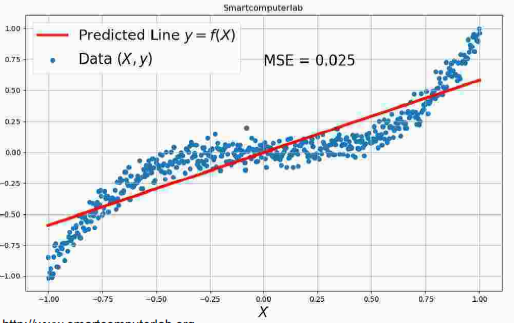
\includegraphics[width=0.6\linewidth]{bias_variance.png}\\
\textbf{Low Bias}
\begin{itemize}
    \item A more complex model can better explain the data
\end{itemize}
\textbf{High Variance}
\begin{itemize}
    \item Given a new datapoint, the MSE can be very large
    \item For a different set with more datapoints, the model may be very different
\end{itemize}
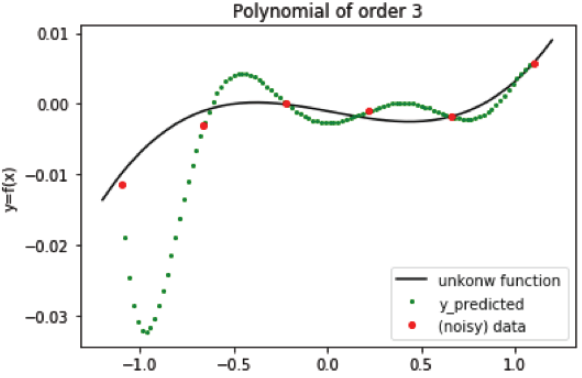
\includegraphics[width=0.6\linewidth]{bias_variance2.png}

\subsubsection{Trade-off}
\begin{itemize}
    \item Higher bias implies lower variance
    \item Lower bias implies higher variance
    \item In practice, all we want is low variance
    \item The model can only be as complex as the data permits
    \item You have to find an optimal balance between bias and variance
\end{itemize}
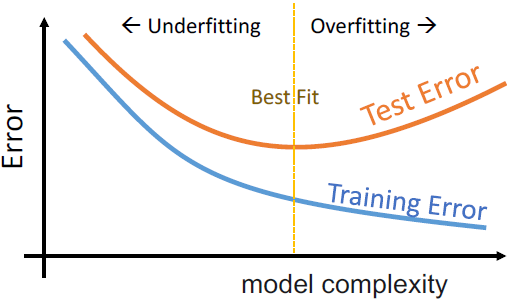
\includegraphics[width=0.6\linewidth]{tradeoff.png}

\subsection{Regularization}
\begin{itemize}
    \item Technique to control the model complexity
    \begin{itemize}
        \item Add a penalty term to the Loss
        \item More complex models get a higher penalty
        \item Add a constrain to the optimization process
        \item \textit{regularized loss} = \textit{MSE + $\lambda$ model-complexity}
    \end{itemize}
\end{itemize}
\begin{center}
    $\displaystyle\sum_{i = 1}^{n} (y_i - \displaystyle\sum_{j = 1}^{p} x_{ij}\beta_j)^2 + \lambda \displaystyle\sum_{j = 1}^{p}\beta_j^2$
\end{center}
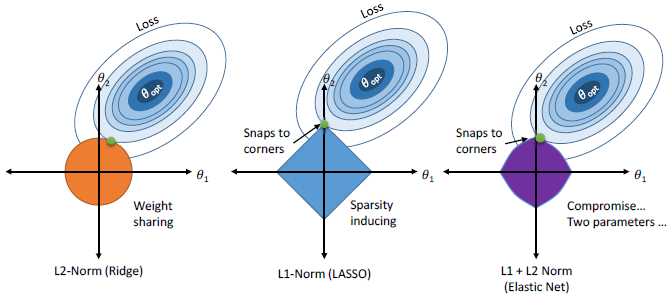
\includegraphics[width=1\linewidth]{regularization.png}
